\section{Background}
\label{sec:background}

\subsection{Blockchain}

At a high level, a blockchain is a sequence of blocks that is difficult to edit, providing practical immutability for the data stored in the blocks.
We choose to view blockchain as a finite state machine where blocks contain data that represent transitions between states of applications running on top of a blockchain, such as cryptocurrency transfers.
Abstractly, the $k^{th}$ block $B_k$ is a transition from state $S_{k-1}$ to state $S_k$ with certain validity requirements.
See Figure \ref{fig:statemachine} for a visual.
Cryptocurrencies realize state as a balance sheet and blocks as sets of transactions that transfer currency between accounts.
Among other validity requirements, no user can have a negative balance and that money cannot be spent twice.

\begin{center}
    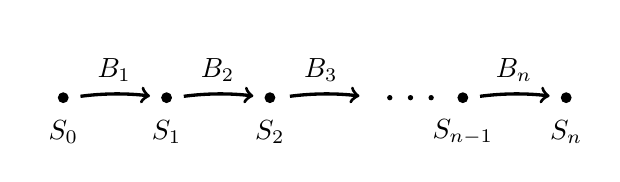
\begin{tikzpicture}[scale=1.75]
        % draw the 0 point
        \draw [thick,color=white] (0,0) -- (0,0);

        % state 0
        \draw [fill=black] (0.25,-0.5) circle (0.035);
        \node at (0.25,-0.75) {$S_0$};

        % block 1
        \draw [very thick, ->] (0.375,-0.49) arc (97.5:83:2);
        \node at (0.62,-0.3) {$B_1$};

        % state 1
        \draw [fill=black] (1,-0.5) circle (0.035);
        \node at (1,-0.75) {$S_1$};

        % block 2
        \draw [very thick, ->] (1.125,-0.49) arc (97.5:83:2);
        \node at (1.37,-0.3) {$B_2$};

        % state 2
        \draw [fill=black] (1.75,-0.5) circle (0.035);
        \node at (1.75,-0.75) {$S_2$};

        % block 3
        \draw [very thick, ->] (1.895,-0.49) arc (97.5:83:2);
        \node at (2.12,-0.3) {$B_3$};

        % ...
        \draw [fill=black] (2.62,-0.5) circle (0.015);
        \draw [fill=black] (2.77,-0.5) circle (0.015);
        \draw [fill=black] (2.92,-0.5) circle (0.015);

        % state n-1
        \draw [fill=black] (3.15,-0.5) circle (0.035);
        \node at (3.15,-0.75) {$S_{n-1}$};

        % block n
        \draw [very thick, ->] (3.275,-0.49) arc (97.5:83:2);
        \node at (3.52,-0.3) {$B_n$};

        % state n
        \draw [fill=black] (3.90,-0.5) circle (0.035);
        \node at (3.90,-0.75) {$S_n$};

    \end{tikzpicture}
    \captionof{figure}{Blocks as transitions between states \label{fig:statemachine}}
\end{center}


\subsection{Technical Problem}

To understand the technical problem, we must understand two properties of blockchains.
First, we observe that miners must have every block in the chain to contribute new blocks.
And, second, blockchains grow in perpetuity.
These properties mean that new miners must download and process an ever increasing amount of data as time passes.
Even now, when Bitcoin is just over a decade old, it can take days or weeks to become a miner.
Such a barrier prevents some nodes from mining, limiting decentralization.
Less decentralization reduces the effectiveness of a blockchain.

When viewing a blockchain as a finite state machine, we can change the requirements of what a miner needs to know.
All a miner must know is a state $S_k$ and every block following that state.
Then a bootstrapping miner could compute the current state.
If $S_k$ is close to the end of the chain, then the miner requires significantly less bootstrapping time by only requesting blocks following $S_k$.

How does a bootstrapping miner obtain the state $S_k$?
They can't just ask a blockchain node, because they could receive a faulty state.
This is the problem we would like to solve: Can we provide a mechanism so that a bootstrapping node can trust a recent state?

\subsection{Related Work}

Our solution gains inspiration from a paper written by Matzutt et al. that provides a way to verify Bitcoin states.
They suggest that recent miners be allowed to vote for a state and then bootstrapping nodes trust the majority of votes.
Each vote is recorded in a block and each block has the capacity to store a single vote \cite{Matzutt2020HowTS}.
Storing votes in blocks gives them immutability, so a bootstrapping node knows that they are counting every vote.

There are two problems with this idea.
First, a vote can only be generated as quickly as new blocks.
In Bitcoin, this averages to about 10 minutes per block, meaning a bootstrapping node might have to wait a week for there to be sufficiently many votes to trust a state.
Second, this solution relies on implementation details in the Bitcoin protocol and may not apply to blockchains in general.

\subsection{Project background}

This project will continue my research from this summer as part of a Research Experiences for Undergraduates (REU) at Montana State University.
My collaborators and I came up with the following idea.

Like Matzutt and his collaborators, we allow recent miners to vote \cite{Matzutt2020HowTS}.
However, we choose to store votes in a distributed hash table.
Storing votes in a distributed hash table is convenient because it allows recent miners to vote immediately, but it also gives attackers an opportunity to delete votes.
To combat vote deletion, we drew on the idea of a tangle \cite{popov2016tangle}.
A tangle is a directed acyclic graph where the nodes are added to tangle by selecting the two most recently added nodes as parents.
In this context, nodes are realized as votes.
A tangle manager receives votes from recent miners and adds each of them to the tangle by attaching them to parent votes.

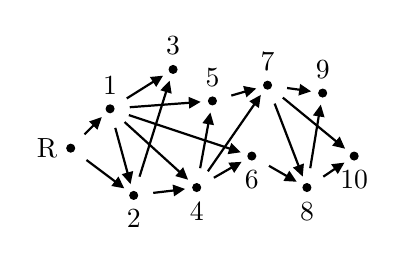
\begin{tikzpicture}[scale=2,rotate=270]
    %% vertices
    \draw [fill=black] (0.0,0.0)     circle (0.025);
    \draw [fill=black] (-0.25,0.25)  circle (0.025);
    \draw [fill=black] (0.3,0.4)     circle (0.025);
    \draw [fill=black] (-0.5,0.65)   circle (0.025);
    \draw [fill=black] (0.25,0.8)    circle (0.025);
    \draw [fill=black] (-0.3,0.9)    circle (0.025);
    \draw [fill=black] (0.05,1.15)   circle (0.025);
    \draw [fill=black] (-0.4,1.25)   circle (0.025);
    \draw [fill=black] (0.25,1.5)    circle (0.025);
    \draw [fill=black] (-0.35,1.6)   circle (0.025);
    \draw [fill=black] (0.05,1.8)    circle (0.025);
    %% labels
    \node at (0.0,-0.15) {R};
    \node at (-0.4,0.25) {1};
    \node at (0.45,0.4) {2};
    \node at (-0.65,0.65) {3};
    \node at (0.4,0.8) {4};
    \node at (-0.45,0.9) {5};
    \node at (0.2,1.15) {6};
    \node at (-0.55,1.25) {7};
    \node at (0.4,1.5) {8};
    \node at (-0.5,1.6) {9};
    \node at (0.2,1.8) {10};
    %% edges
    \draw [thick] (-0.088,0.088) -- (-0.162,0.162);
    \draw [thick] (0.075,0.1) -- (0.225,0.3);
    \draw [thick] (-0.129,0.283) -- (0.179,0.367);
    \draw [thick] (-0.316,0.356) -- (-0.434,0.544);
    \draw [thick] (-0.166,0.342) -- (0.166,0.708);
    \draw [thick] (-0.26,0.375) -- (-0.29,0.775);
    \draw [thick] (-0.21,0.369) -- (0.01,1.031);
    \draw [thick] (0.181,0.437) -- (-0.381,0.613);
    \draw [thick] (0.284,0.524) -- (0.266,0.676);
    \draw [thick] (0.127,0.822) -- (-0.177,0.878);
    \draw [thick] (0.188,0.909) -- (0.112,1.041);
    \draw [thick] (0.147,0.871) -- (-0.297,1.179);
    \draw [thick] (-0.334,1.02) -- (-0.366,1.13);
    \draw [thick] (0.112,1.259) -- (0.188,1.391);
    \draw [thick] (-0.283,1.295) -- (0.133,1.455);
    \draw [thick] (-0.382,1.374) -- (-0.368,1.476);
    \draw [thick] (-0.321,1.347) -- (-0.029,1.703);
    \draw [thick] (0.127,1.521) -- (-0.227,1.579);
    \draw [thick] (0.181,1.604) -- (0.119,1.696);
    %% arrows
    \fill [black] (-0.197,0.197) -- (-0.117,0.17) -- (-0.17,0.117);
    \fill [black] (0.255,0.34) -- (0.24,0.258) -- (0.18,0.303);
    \fill [black] (0.228,0.38) -- (0.165,0.324) -- (0.145,0.397);
    \fill [black] (-0.46,0.586) -- (-0.389,0.543) -- (-0.452,0.503);
    \fill [black] (0.2,0.745) -- (0.177,0.664) -- (0.121,0.714);
    \fill [black] (-0.294,0.825) -- (-0.251,0.753) -- (-0.326,0.748);
    \fill [black] (0.026,1.079) -- (0.038,0.996) -- (-0.033,1.02);
    \fill [black] (-0.428,0.628) -- (-0.346,0.641) -- (-0.368,0.569);
    \fill [black] (0.259,0.726) -- (0.306,0.656) -- (0.231,0.647);
    \fill [black] (-0.226,0.887) -- (-0.146,0.91) -- (-0.159,0.836);
    \fill [black] (0.087,1.085) -- (0.157,1.038) -- (0.092,1.001);
    \fill [black] (-0.338,1.207) -- (-0.255,1.195) -- (-0.298,1.134);
    \fill [black] (-0.379,1.178) -- (-0.323,1.116) -- (-0.395,1.095);
    \fill [black] (0.213,1.435) -- (0.208,1.351) -- (0.143,1.388);
    \fill [black] (0.18,1.473) -- (0.123,1.411) -- (0.097,1.481);
    \fill [black] (-0.361,1.526) -- (-0.334,1.446) -- (-0.408,1.457);
    \fill [black] (0.003,1.742) -- (-0.016,1.66) -- (-0.074,1.708);
    \fill [black] (-0.276,1.588) -- (-0.196,1.612) -- (-0.208,1.538);
    \fill [black] (0.092,1.738) -- (0.164,1.696) -- (0.102,1.654);
\end{tikzpicture}

A vote is invalid if one if its parents is invalid or deleted.
Deleting a vote causes a chain reaction in the tangle that deletes votes that support the attacker, preventing the attacker from swinging the election, by disproportionately deleting votes on one side of the election.
A bootstrapping node can request the vote tangle and then make a decision based on valid votes.

While we do have a sketch of a solution idea, more work needs to be done to prove its correctness and security as well as to demonstrate these properties through a practical implementation.
Preliminary results indicate that it is resistant to some types of attacks but we need to consider smarter and more powerful attackers.
